% UI functions: RetrievalPage.tsx, ExperimentPanel.tsx; routers/chat.py; session_store.py.
% Sources: configs/config.yaml; .env.example (sample only); chat_service.py;
% retrieval_service.py; agents/rag_agent.py; model_gateway.py; ingestion/chunker.py.
% Sparse scoring: indexing/learned_sparse_index.py, LearnedSparseIndex.query.
\section{Thiết kế và hiện thực hệ thống}
\subsection{Kiến trúc và luồng xử lý}
Hệ thống tổ chức theo mô hình client--server. Backend sử dụng FastAPI để tiếp nhận câu hỏi và điều phối xử lý; frontend React/TypeScript hiển thị hội thoại, trạng thái xử lý và các đoạn nguồn.
\par
\begin{figure}[H]\centering
\begin{tikzpicture}[node distance=0.6cm and 0.4cm]
\node[box] (a) {Frontend React\\Hội thoại và nguồn};
\node[box,right=of a] (b) {Backend FastAPI\\Phiên và dịch vụ chat};
\node[box,right=of b] (f) {Cổng gọi mô hình\\Provider theo cấu hình};
\node[box,below=of a] (c) {Bộ thực nghiệm\\Chia tập, lưu và chấm điểm};
\node[box,right=of c] (d) {Lõi RAG dùng chung\\Truy xuất, xếp hạng, sinh};
\node[box,right=of d] (e) {Kho bài báo và chỉ mục\\Sparse / Chroma dense};
\draw[flow] (a)--(b);\draw[flow] (b)--(d);\draw[flow] (b)--(f);\draw[flow] (c)--(d);\draw[flow] (e)--(d);\draw[flow] (d.north east)--(f.south west);
\end{tikzpicture}
\caption[Kiến trúc ứng dụng và bộ thực nghiệm chính.]{Kiến trúc ứng dụng và bộ thực nghiệm chính. Mũi tên từ kho cung cấp dữ liệu; các mũi tên còn lại thể hiện yêu cầu xử lý.}\label{fig:architecture}
\end{figure}

\par
Ứng dụng và bộ thực nghiệm chính dùng chung lõi truy xuất, xếp hạng lại và sinh câu trả lời. Bộ thực nghiệm bổ sung chia tập, lưu kết quả và chấm điểm.

Ứng dụng ưu tiên bộ chỉ mục sparse đã khóa nếu có đủ dữ liệu đoạn và tệp chỉ mục; nếu thiếu, hệ thống thử truy xuất qua Chroma dense. Nhánh sparse dùng chỉ mục đảo; điểm truy xuất là tổng các tích trọng số BGE-M3 trên những token chung của câu hỏi và đoạn văn.

Mô hình và chỉ mục được tải khi cần rồi lưu trong bộ nhớ; lỗi khởi tạo được chuyển về tầng chat.

\begin{itemize}
\item \textbf{Truy vấn RAG:} backend lấy ứng viên, xếp hạng lại, chọn số đoạn ngữ cảnh rồi gọi mô hình sinh. Truy xuất dùng câu hỏi hiện tại; nhánh chat trực tiếp gửi cả lịch sử hội thoại cho mô hình.
\item \textbf{Hiển thị nguồn:} ưu tiên các đoạn được dẫn trong câu trả lời. Nếu không có dẫn nguồn hợp lệ, giao diện hiển thị danh sách sau xếp hạng lại; danh sách này có thể chứa đoạn chưa được đưa cho mô hình khi độ sâu ngữ cảnh nhỏ hơn số đoạn giữ lại.
\end{itemize}
\par
\begin{figure}[H]\centering
\begin{tikzpicture}[node distance=0.8cm and 1cm]
\node[box] (a) {Câu hỏi và cấu hình\\Chọn chế độ chat};
\node[box,right=of a] (b) {Truy xuất ứng viên\\Xếp hạng lại};
\node[box,below=of a] (e) {Gọi mô hình trực tiếp\\Câu hỏi và lịch sử chat};
\node[box,below=of b] (c) {Gọi mô hình theo RAG\\Lời nhắc và các đoạn đã chọn};
\node[box,below=of e] (d) {Hiển thị câu trả lời\\Kèm nguồn nếu có};
\draw[flow] (a)--node[above,font=\footnotesize]{RAG}(b);
\draw[flow] (a)--node[left,font=\footnotesize]{Trực tiếp}(e);
\draw[flow] (b)--(c);
\draw[flow,dashed] (b.south west)--node[midway,fill=white,inner sep=1pt,sloped,font=\footnotesize]{Lỗi}(e.north east);
\draw[flow,dashed] (c.west)--node[above,fill=white,inner sep=1pt,font=\footnotesize]{Lỗi}(e.east);
\draw[flow] (e)--(d);
\draw[flow] (c.south)|-(d.east);
\end{tikzpicture}
\caption{Luồng xử lý truy vấn và nhánh chat dự phòng}\label{fig:query}
\end{figure}

\par
\subsection{Cấu hình ứng dụng}
Bảng~\ref{tab:system} tóm tắt các giá trị khai báo và nhánh áp dụng. Ký hiệu 512/64 chỉ kích thước 512 token với phần chồng lấp 64 token; 256/32 được hiểu tương tự. Giá trị trong cấu hình, môi trường mẫu và mặc định trong mã có vai trò khác nhau.
\begin{table}[H]\setstretch{1.05}\centering\caption{Cấu hình hệ thống và nhánh áp dụng}\label{tab:system}\small
\begin{tabularx}{\linewidth}{@{}P{1.65cm}Y Y@{}}\toprule
\textbf{Nhóm} & \textbf{Giá trị khai báo} & \textbf{Vai trò và nhánh áp dụng}\\\midrule
Chunking & Recursive 512/64; \code{cl100k_base}; đoạn con 256/32 & Đo bằng token; phân cấp tìm đoạn con, chuyển đoạn cha 512/64 cho tầng sinh \\
Sparse & BGE-M3, \code{BAAI/bge-m3}; top-k 20 & Learned-sparse; 20 ứng viên cho reranker; không dùng HNSW \\
Dense & \code{all-MiniLM-L6-v2}, 384 chiều; cosine & Chroma; nhánh truy xuất theo độ tương tự vector \\
Reranker & \code{BAAI/bge-reranker-large}; top-n 5; batch 8 & Cross-encoder xếp hạng lại các ứng viên đã truy xuất \\
Sinh đáp án & Gemini 3.1 Flash-Lite; P2; 5 đoạn; $T=0$; tối đa 512 token; reasoning minimal & Prompt/số đoạn từ pipeline; tham số sinh từ thiết lập chat \\
Lưu trữ & \code{data/locked_index}; \code{data/chroma_db}; collection \code{newsqa_cnn} & Sparse tách khỏi Chroma; môi trường có thể đổi đường dẫn và collection \\
Vận hành & Môi trường mẫu: rag, lịch sử 20, \code{RAG_TOP_K=5} & Mặc định trong mã là auto; khi RAG lỗi có thể chuyển sang chat trực tiếp \\\bottomrule
\end{tabularx}\end{table}

Biến môi trường được ưu tiên hơn giá trị trong tệp môi trường; dịch vụ chat lấy tham số sinh từ môi trường hoặc mặc định trong mã. Pipeline xác định prompt, số ứng viên và độ sâu. Thiết lập mẫu lấy 20 ứng viên ở nhánh sparse, 5 ở nhánh Chroma và gửi tối đa 5 đoạn cho mô hình sinh.
\subsection{Chức năng}
\begin{itemize}
\item \textbf{Hỏi đáp:} hiển thị câu trả lời, nguồn và lịch sử theo phiên; cho phép xem hoặc xóa hội thoại. Backend dùng Server-Sent Events để gửi trạng thái và kết quả cuối, chưa truyền từng token đang sinh.
\item \textbf{Thử truy xuất:} chọn thuật toán, số kết quả và xem đoạn cùng thời gian xử lý.
\item \textbf{Thực nghiệm:} xem cấu hình, chạy hoặc tiếp tục thực nghiệm và nạp báo cáo kết quả.
\end{itemize}
\subsection{Vận hành và kiểm thử}
Dịch vụ chat kiểm tra cấu hình trước khi xử lý và trả thông báo tổng quát khi gặp lỗi. Nhánh chat dự phòng không dùng bằng chứng từ kho tin.

Bộ kiểm thử dùng dữ liệu mẫu và thành phần giả lập để kiểm tra cấu hình, truy xuất, dẫn nguồn, chia đoạn, chấm điểm và tiếp tục lần chạy. Phụ lục~\ref{app:reproduction} nêu cách cài đặt và kiểm thử; chất lượng mô hình được đánh giá ở Chương 5.

\subsection{Minh họa giao diện}
Hình~\ref{fig:app-chat} minh họa câu hỏi về tay golf Henrik Stenson, câu trả lời và đoạn nguồn CNN. Thông tin nguồn được lấy từ metadata của bài báo.
\begin{figure}[H]
\centering
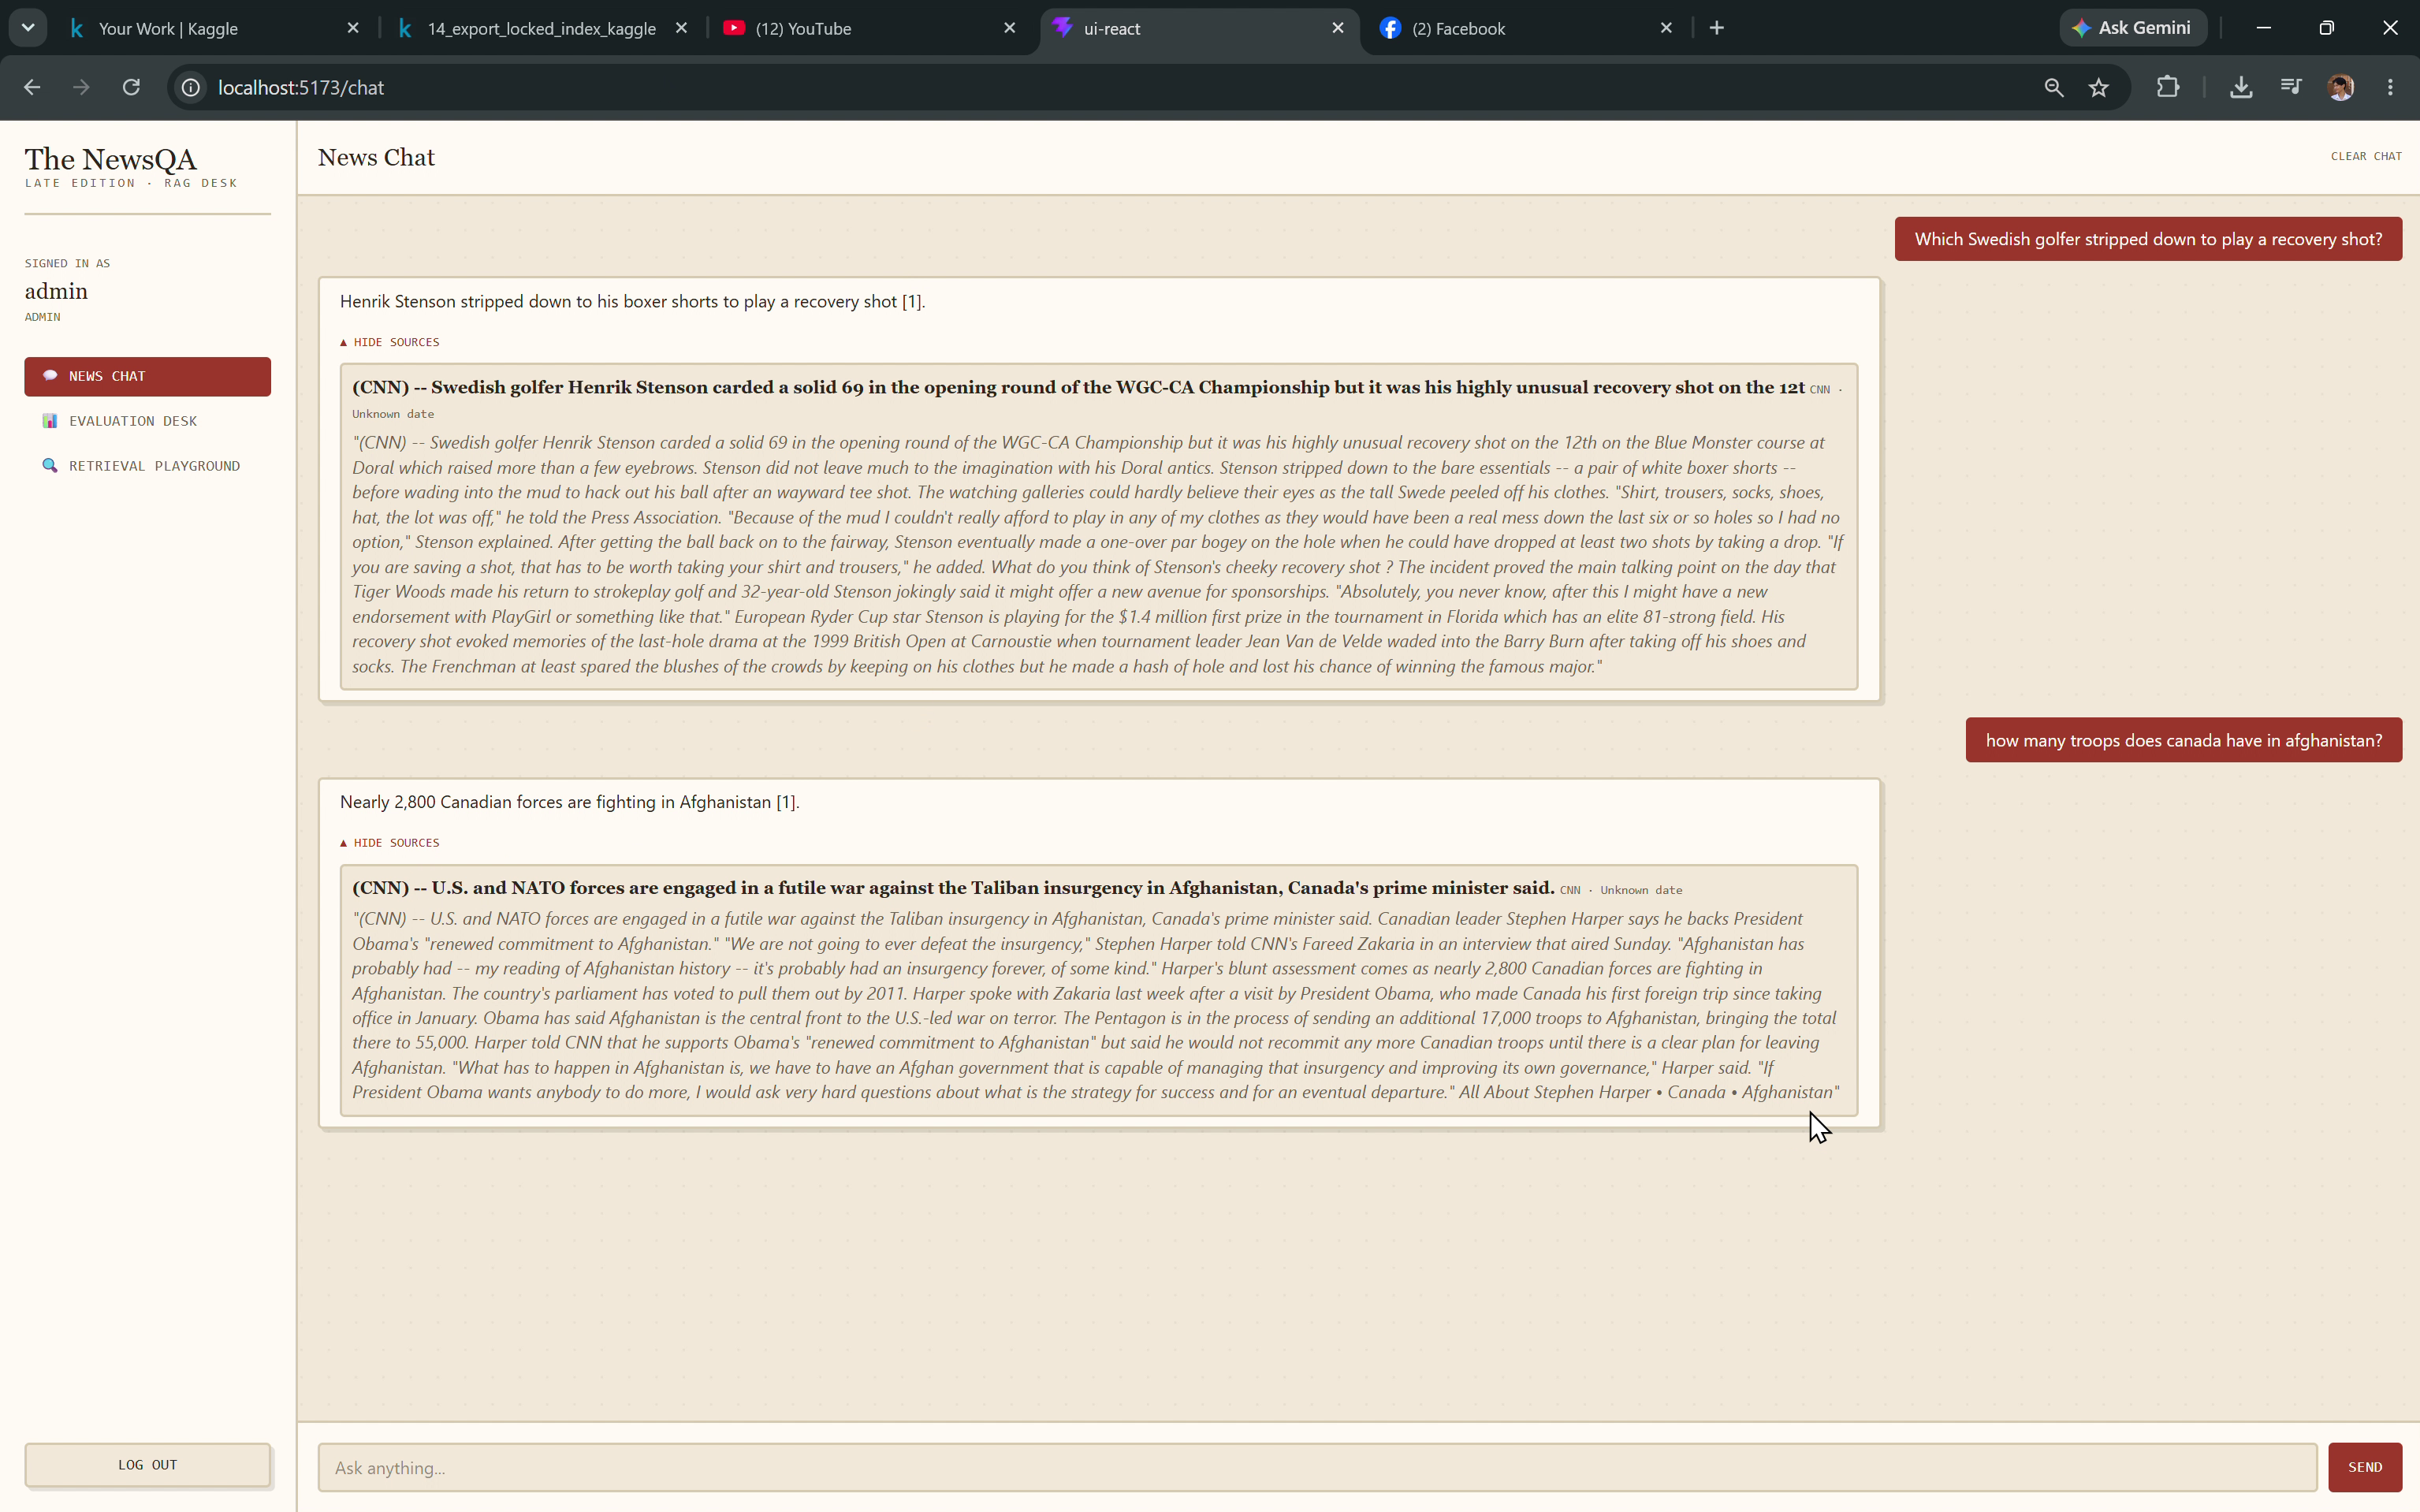
\includegraphics[width=0.98\linewidth,trim=375bp 1018bp 20bp 260bp,clip]{../figures/chat_interface.png}
\par\vspace{3pt}
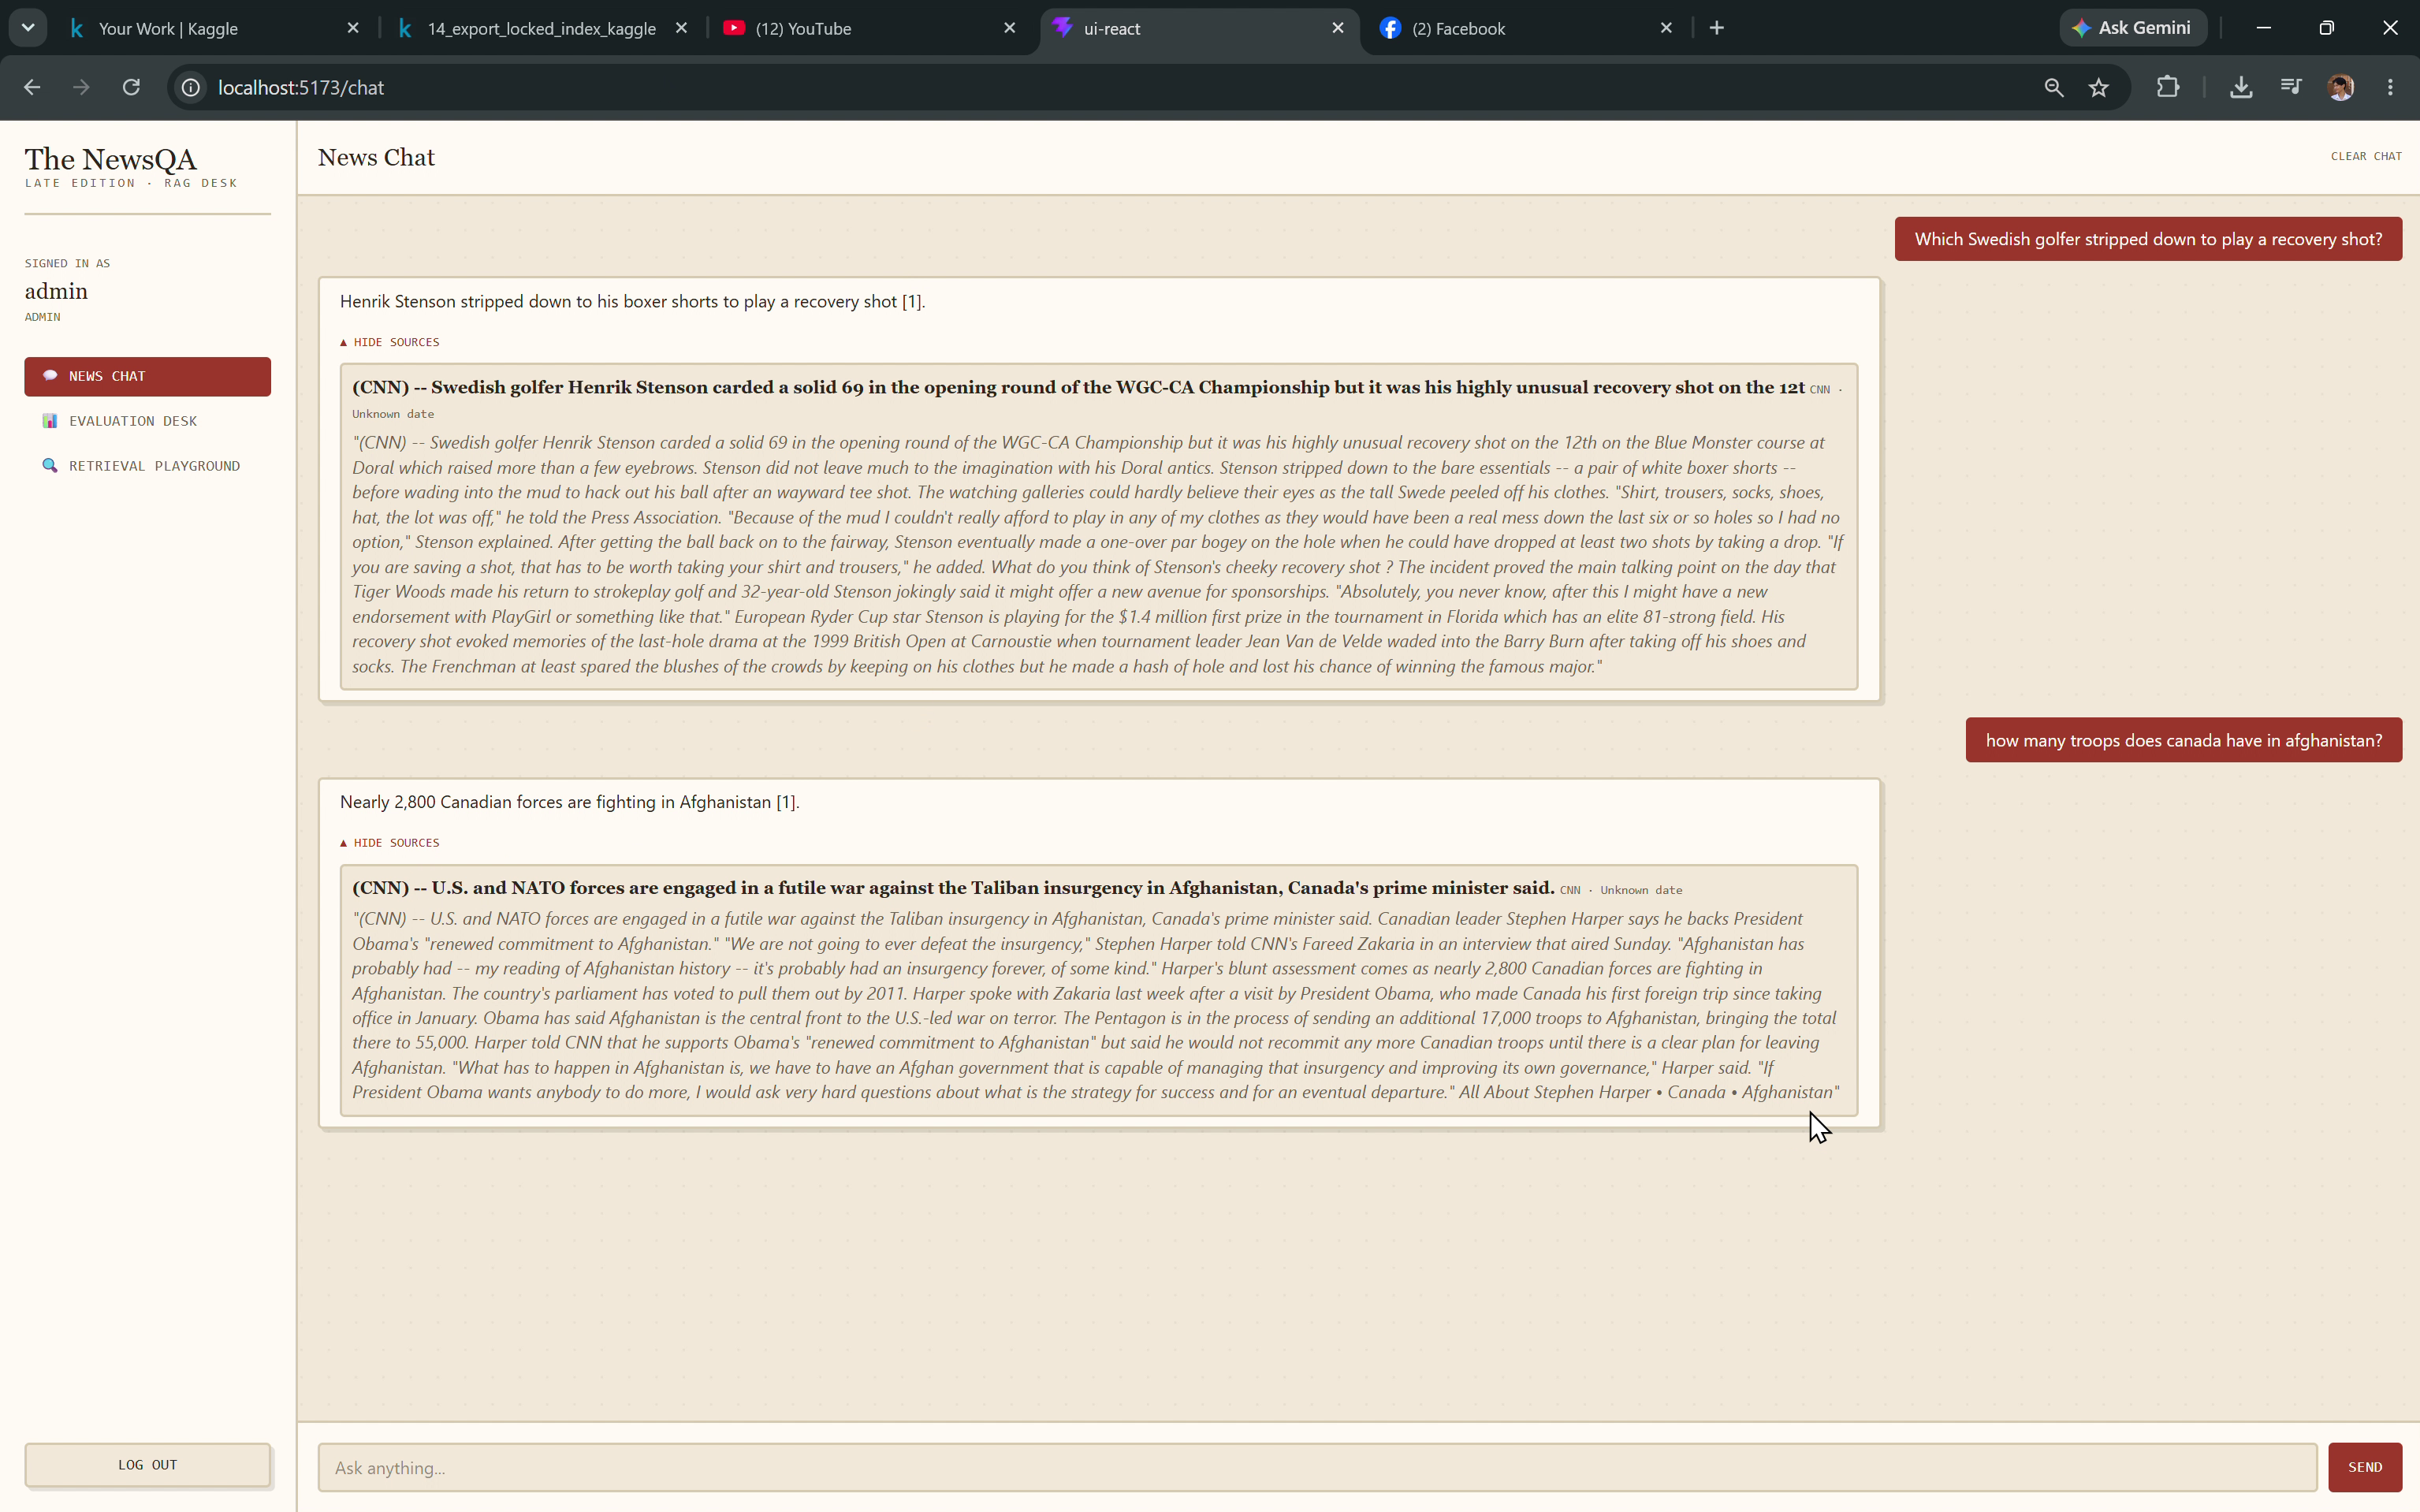
\includegraphics[width=0.85\linewidth,trim=400bp 1500bp 1850bp 350bp,clip]{../figures/chat_interface.png}
\caption[Hỏi đáp và dẫn nguồn trên giao diện.]{Hỏi đáp và đoạn nguồn CNN; phía dưới phóng lớn câu trả lời cùng chỉ dấu nguồn.}\label{fig:app-chat}
\end{figure}
Hình~\ref{fig:app-retrieval} minh họa lựa chọn thuật toán và kết quả truy xuất. Bộ sưu tập Chroma 323 đoạn trong ảnh thuộc lần chạy minh họa, khác chỉ mục sparse dùng cho thực nghiệm ở Chương 5.
\begin{figure}[H]
\centering
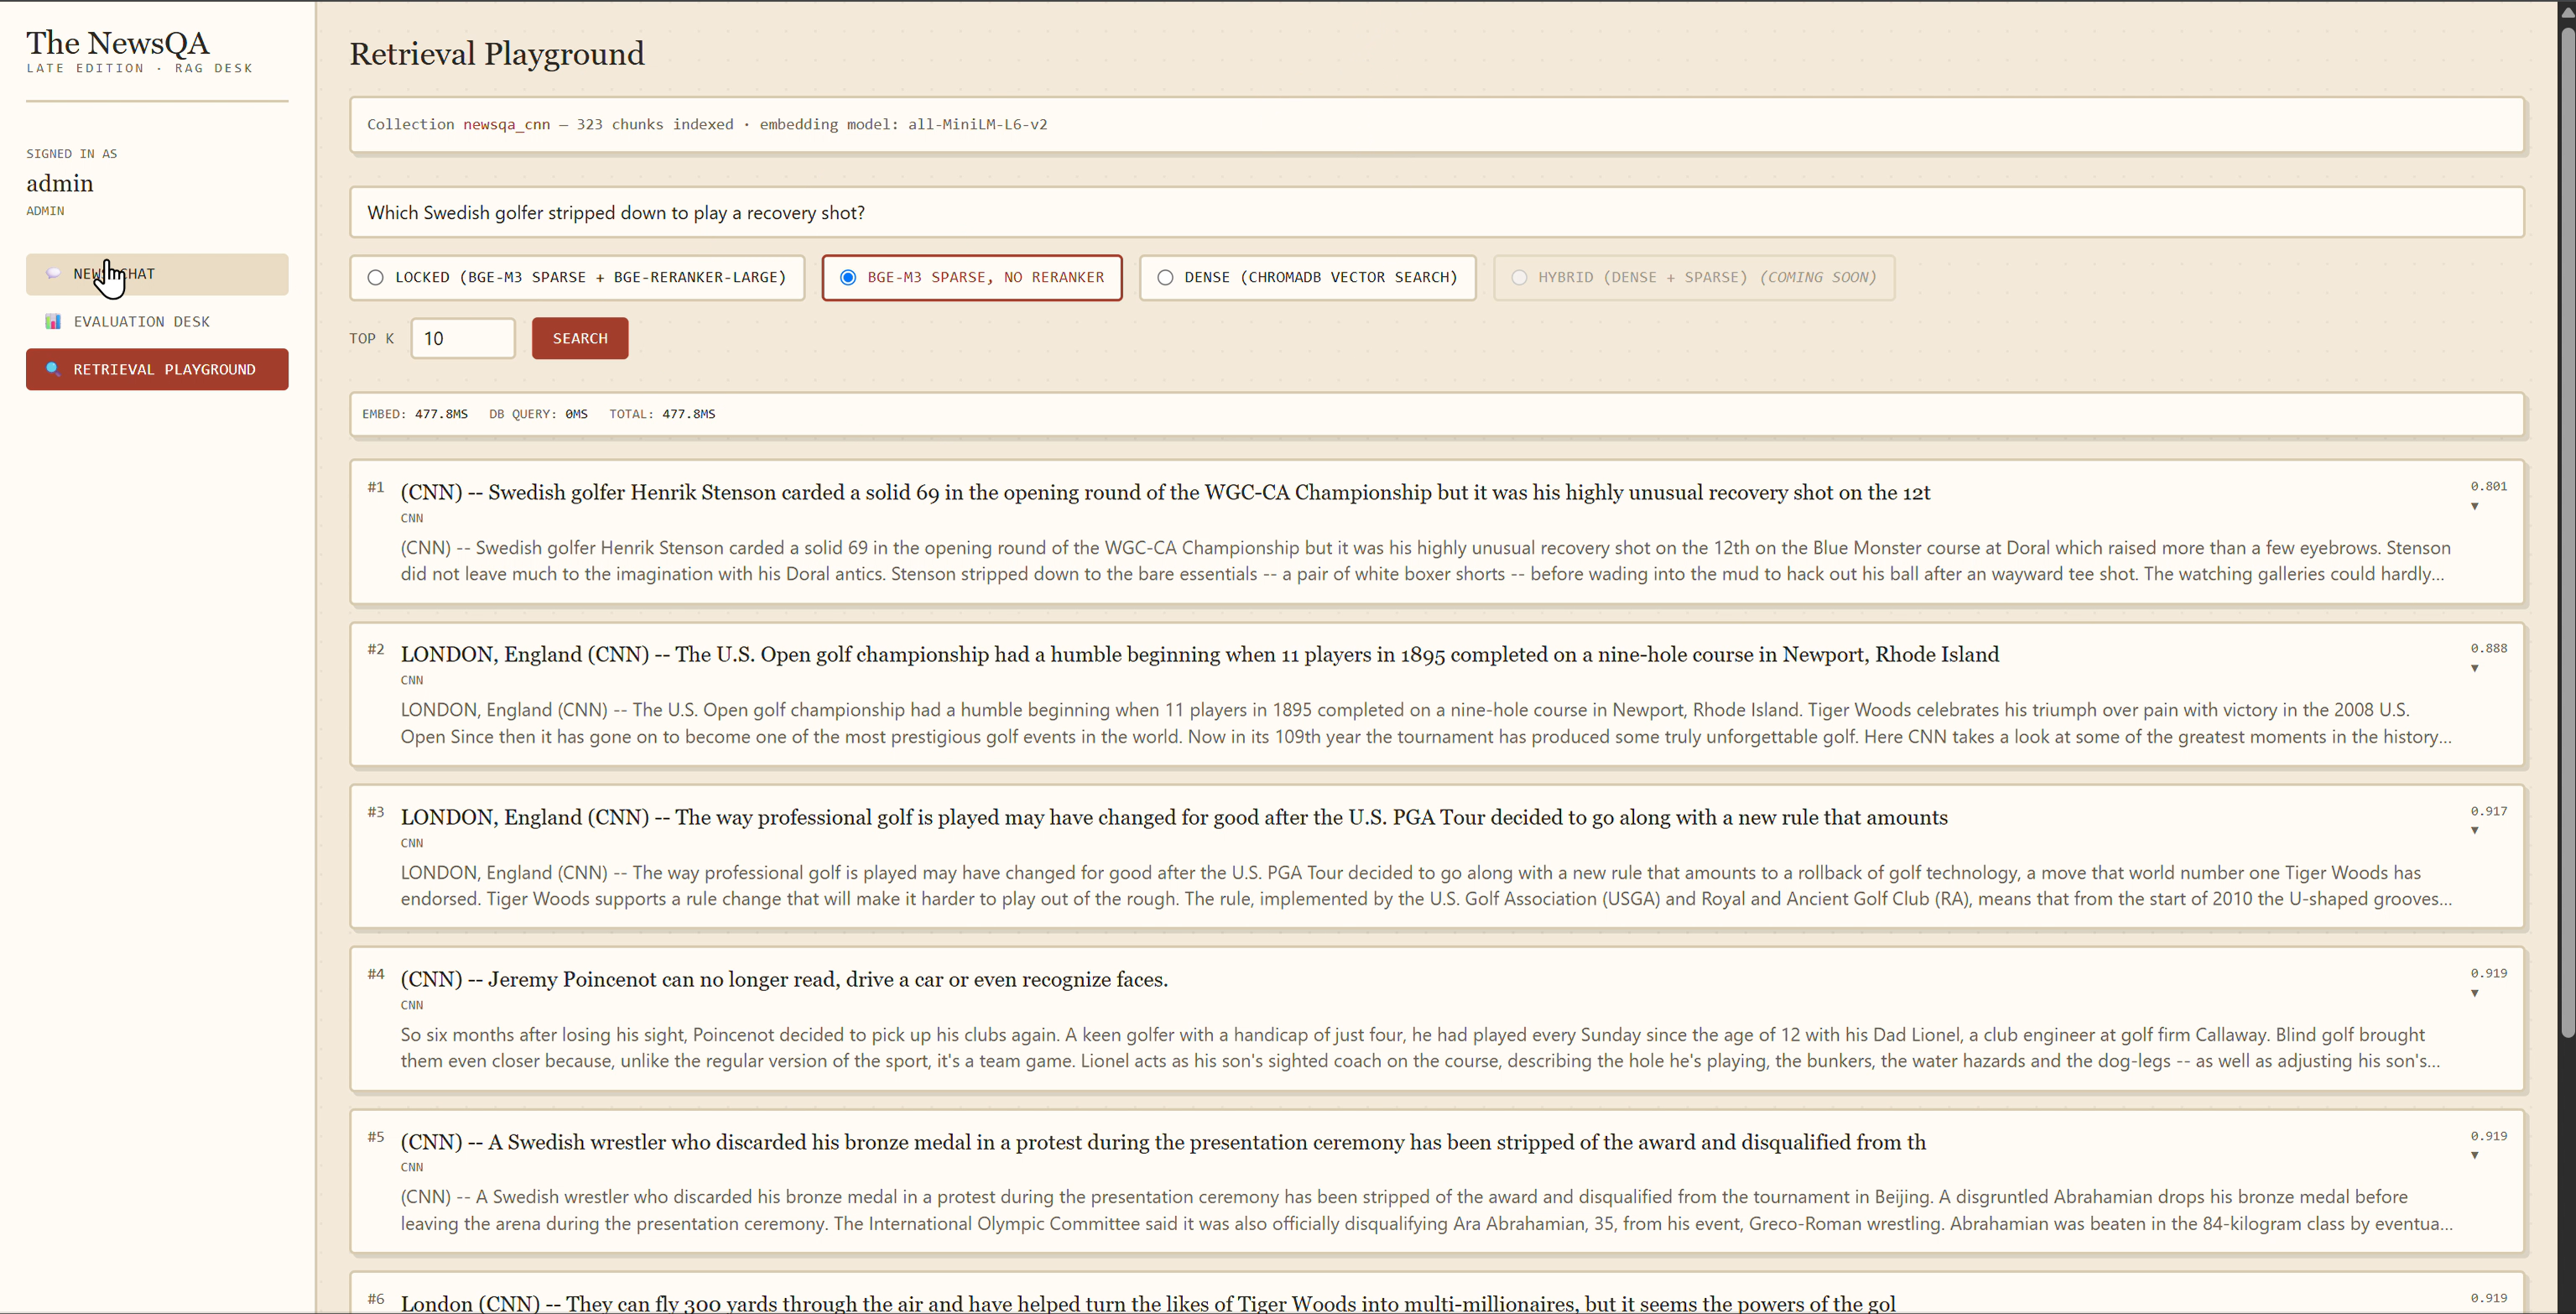
\includegraphics[width=0.98\linewidth,trim=171.43bp 359.15bp 21.43bp 45bp,clip]{../figures/retrieval_playground.png}
\par\vspace{3pt}
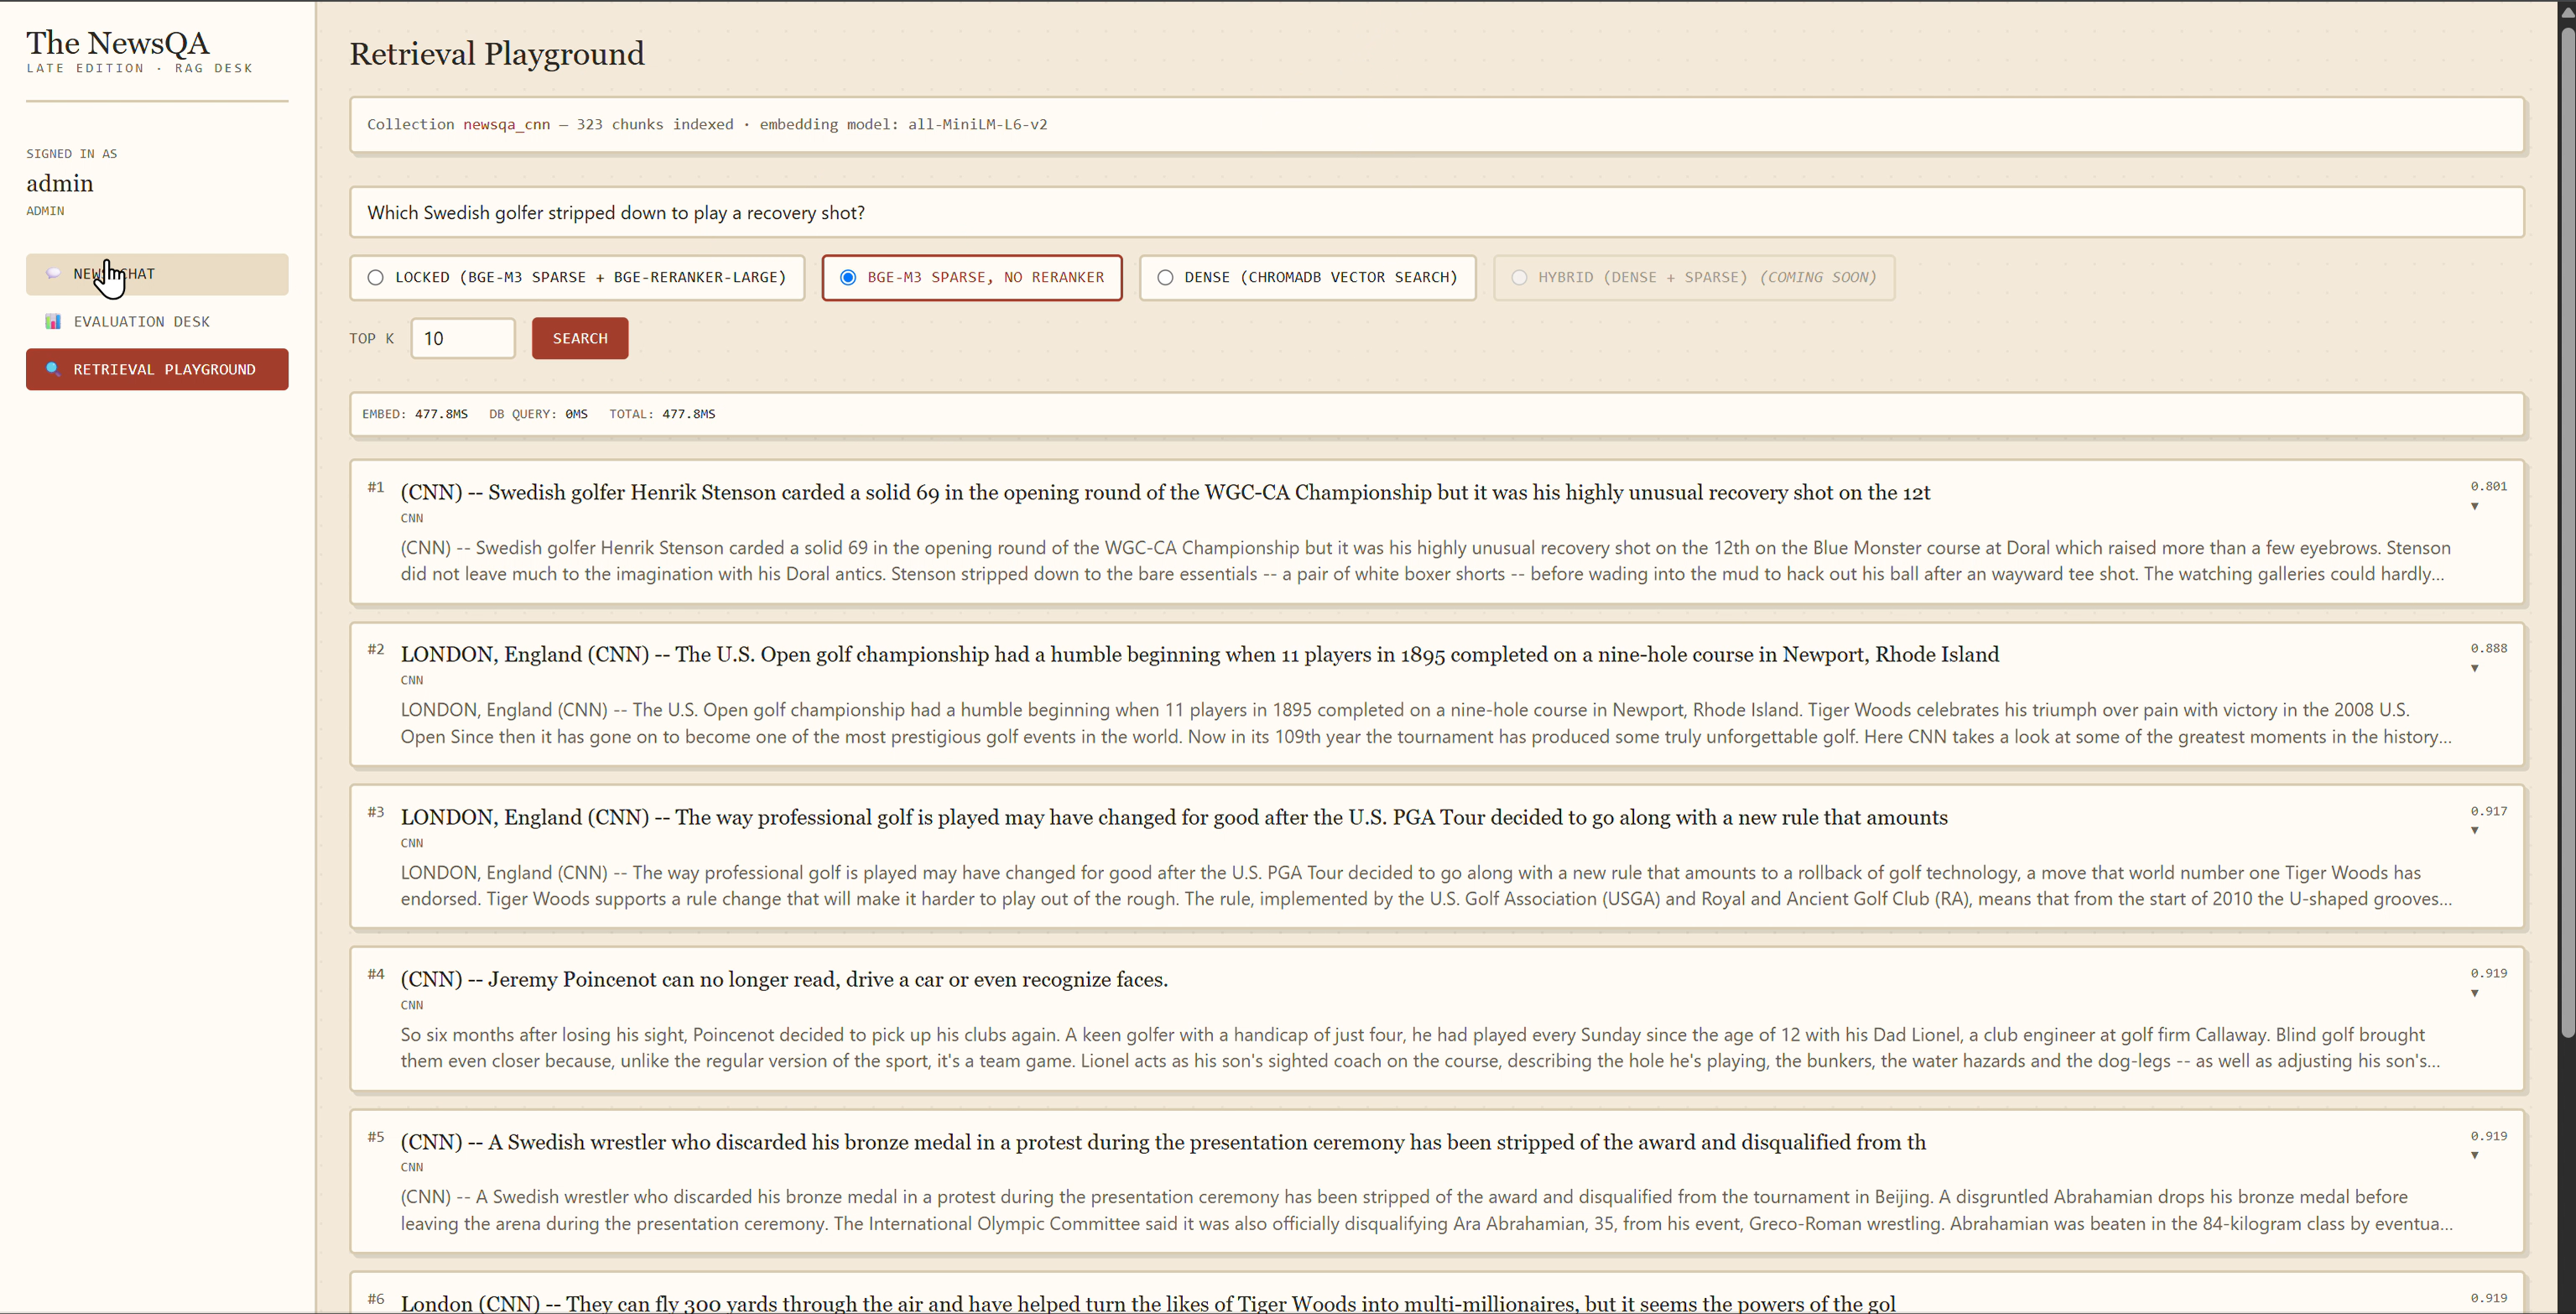
\includegraphics[width=0.48\linewidth,trim=418.72bp 518.58bp 737.15bp 128.57bp,clip]{../figures/retrieval_playground.png}
\caption[Thử truy xuất và kết quả đầu tiên.]{Thử truy xuất và kết quả đầu tiên; phía dưới phóng lớn thuật toán đang chọn.}\label{fig:app-retrieval}
\end{figure}
